\section{The Canonical Decomposition-Recombination Plan}
\label{sec:DRP}

\newcommand{\usestwod}{\todo{Uses 2D requirement:}}
\renewcommand{\usestwod}{}

\subsection{Theory}

In the problem of the optimal DR-Plan there is generally not a unique plan.
% Indeed, we will prove a union of $N$ well-constrained subgraphs will result in $N$ unique plans, but that at the $N^{\text{th}}$ level of the tree it will always be the same. Therefore, all choices of decomposition are in some sense equivalent. The theorem we seek to prove is thus:
However, we will show that regardless of which children are chosen for the plan, so long as they satisfy the definition of an optimal DR-plan, the recombination will require solving of the same systems. Being the smallest such structure that offers this, the definition of an optimal DR-plan could be considered the canonical DR-plan.
% To assist in showing this, we prove this core theorem throughout this section:

In this section, we discuss 2D bar-joint graphs. All vertex weights are $2$, all edge weights are $1$, and constant $k= -{{3}\choose{2}}=-3$. Trivial graphs are a single vertex and empty set. Furthermore, 2D well-constrained graphs must be connected.
% The greatest density of a 2D well-constrained graph is $-2$ (the vertex). The other disconnected part of the graph would need to have a density of $-1$, which is over-constrained and not possible in a well-constrained graph (because there is no trivial graph with that density).



\begin{theorem}\label{theorem:main}
Given a well-constrained 2-dimensional bar-joint graph $G$, for node $C$ in $OptimalDRP(G)$ and the children of $C$ in $CompleteDRP(C)$ labeled as $C_1,\ldots,C_N$
\begin{enumerate}
    \item if $C_i \cap C_j$ is trivial then all $C_1,\ldots,C_N$ are children of $C$ in $OptimalDRP(G)$
    \item if $C_i \cap C_j$ is well-constrained then any two out of $C_1,\ldots,C_N$ will be the only children of $C$ in $OptimalDRP(G)$.
\end{enumerate}
This covers all potential cases.
\end{theorem}

\begin{proof}
Remark \ref{lemma:union_intersection} shows that the intersection of any two well-constrained subgraphs (such as $C_i$ and $C_j$) can only result in trivial or well-constrained subgraphs. Therefore, these are the only possibilities to consider.

\medskip\noindent
\vemph{Part 1:} We show that no subset of the children can union to form $C$, thereby requiring all of them be included in an optimal plan.

Take the strict subset $S\subsetneq \{1,\ldots,N\}$ such that $U=\bigcup_{i\in S}{C_i}$ which we \vemph{assume} is well-constrained. If $U\neq C$, then we just found a larger proper subgraph and the children were not vertex-maximal to begin with. So, it must be that $U=C$.
\usestwod
However, since $C_i \cap C_j$ is trivial then for $k\notin S$ we know, by Lemma \ref{lemma:uc_intersection_makes_all_uc}, $U\cap C_k$ must be one or more trivial subgraphs. By definition of a DR-plan $C_k=C\cap C_k$ and we know that $U=C$ so $C_k=U\cap C_k$. Thus, $C_k$ is both one or more trivial subgraphs and a well-constrained subgraph of $C$. Thus, the assumption is wrong and $U$ cannot be well-constrained. As $C$ is well-constrained, this means no proper subset of the children in $CompleteDRP(C)$ can union to form $C$.

\medskip\noindent
\vemph{Part 2:} If $C_i \cap C_j$ is well-constrained, then, by Remark \ref{lemma:union_intersection}, $C_i \cup C_j$ is also well-constrained. This means that, by Lemma \ref{lemma:wc_intersection_makes_all_wc}, any two children of $C$ will union to $C$ itself. Thus, any two children are potential choices for the optimal DR-plan as they all create equal fan-in (exactly two) at this level.

However, to guarantee that any two are \vemph{solutions} to $OptimalDRP(G)$, it must ensure minimum fan-in for any descendant. Take the set $S_N=\{1,\dots,N\}$, then we call $I=\bigcap_{k\in S_N}{C_k}$ and $R_k=C\setminus C_k$. Suppose we select $i$ and $j$, where $i\neq j$, as the children. Since
% \[C_i=Idc\left(C,I\cup\bigcup_{k\in S_N\setminus\{i\}}{R_k}\right)\]
% the children of this node will be
% \[Idc\left(C,I\cup\bigcup_{k\in S_N\setminus\{i,m\}}{R_k}\right)\]
% and
% \[Idc\left(C,I\cup\bigcup_{k\in S_N\setminus\{i,n\}}{R_k}\right)\]
$C_i=Idc\left(C,I\cup\bigcup_{k\in S_N\setminus\{i\}}{R_k}\right)$
the children of this node will be
$Idc\left(C,I\cup\bigcup_{k\in S_N\setminus\{i,m\}}{R_k}\right)$
and
$Idc\left(C,I\cup\bigcup_{k\in S_N\setminus\{i,n\}}{R_k}\right)$
for arbitrary $m$ and $n$, where $i,j,m,n$ do not equal each other. \todo{Prove these are valid children? Or is this obvious?} This continues for $N-1$ levels total, always with fan-in of two (the minimum possible), at which point every descendant of $C$ is some $Idc(C,I\cup R_k)$ for $k\in S_N$, with every $k$ appearing at least once. Thus, regardless of the choice of $i,j$ and then $m,n$ etc., the DR-plan has fan-in of two for every node for the next $N$ levels, at which point the nodes contain the same subgraphs.

This proof then applies to itself recursively to show that the fan-in of the children will also be minimum, thereby making this the optimal DR-plan.
\end{proof}

% The following subsections provide the supporting proofs.



%%%%%%%%%%%%%%%%%%%%%%%%%%%%%%%%%%%%%%%%%%%%%%%%%%%%%%%%%%%%%%%%
%%%%%%%%%%%%%%%%%%%%%%%%%%%%%%%%%%%%%%%%%%%%%%%%%%%%%%%%%%%%%%%%
%%%%%%%%%%%%%%%%%%%%%%%%%%%%%%%%%%%%%%%%%%%%%%%%%%%%%%%%%%%%%%%%

% \subsubsection{Relationships for the Union and Intersection of Well-Constrained Subgraphs}
% \label{sec:union_intersection}

% This is general, not for 2d
\begin{remark}\label{lemma:union_intersection}
If $F_i$ and $F_j$ are well-constrained subgraphs of the same well-constrained graph $F$, then it must be that: (1) $F_i\cup F_j$ is not trivial; (2) $F_i\cup F_j$ is under-constrained if and only if $F_i\cap F_j$ is trivial; (3) $F_i\cup F_j$ is well-constrained if and only if $F_i\cap F_j$ is well-constrained; and (4) $F_i\cap F_j$ is not under-constrained.
\end{remark}

\begin{proof}
For (1), simply note that if $F_i\cup F_j$ were trivial, then, by definition, $F_i$ and $F_j$ must be trivial.

For (2), observe that under-constrained subgraphs of well-constrained graphs must have density less than $k$. For (3), observe that, given a well-constrained graph, a subgraph with density $k$ must also be well-constrained. Then, use the fact that, by definition, $d(F_i)=k$ and $d(F_j)=k$. Then it is straightforward application of the equation $d(F_i\cap F_j)=d(F_i)+d(F_j)-d(F_i\cup F_j)$.

For (4), because subgraphs of a well-constrained graph can only be trivial, under-, or well-constrained, all cases have already been exhausted.
\end{proof}

% \begin{proof}
% Use the fact that, by definition, $d(F_i)=k$ and $d(F_j)=k$. Also, the equation $d(F_i\cap F_j)=d(F_i)+d(F_j)-d(F_i\cup F_j)$.
% \begin{enumerate}
%     \item If $F_i\cup F_j$ were trivial, then, by definition, $F_i$ and $F_j$ must be trivial.

%     \item Observe that  Then it is straightforward application of the equation above.

%     % \item Observe that, given a well-constrained graph, an under-constrained subgraph must have density less than $k$. Then it is straightforward application of the equation above.

%     \item Observe that, given a well-constrained graph, a subgraph with density $k$ must also be well-constrained. Then it is straightforward application of the equation above.

%     % \item \textit{Forward direction:} Since $F_i\cup F_j$ is under-constrained and a subgraph of well-constrained $F$, it must be that $d(F_i\cup F_j)=l<k$. Therefore $d(F_i\cap F_j)=2k-l>k$. This means $F_i\cap F_j$ is trivial. \textit{Reverse direction:} We know that $d(F_i\cap F_j)>k$ because it is trivial. By the same math, we find that $d(F_i\cup F_j)<k$, showing it is under-constrained.

%     % \item \textit{Forward direction:} We have that $d(F_i\cup F_j)=k$, therefore $d(F_i\cap F_j)=k$. Being a subgraph of well-constrained $F$, $F_i\cap F_j$ is also well-constrained. \textit{Reverse direction:} By the same math, we find that $d(F_i\cup F_j)=k$ and, since it is also a subgraph of $F$, it is well-constrained.

%     \item Subgraphs of a well-constrained graph can only be trivial, under-, or well-constrained. All cases are already exhausted.
% \end{enumerate}
% \end{proof}





%%%%%%%%%%%%%%%%%%%%%%%%%%%%%%%%%%%%%%%%%%%%%%%%%%%%%%%%%%%%%%%%
%%%%%%%%%%%%%%%%%%%%%%%%%%%%%%%%%%%%%%%%%%%%%%%%%%%%%%%%%%%%%%%%
%%%%%%%%%%%%%%%%%%%%%%%%%%%%%%%%%%%%%%%%%%%%%%%%%%%%%%%%%%%%%%%%

% \subsubsection{Inferring Parent Structure from Union and Intersection of Children}
% \label{sec:infer_parent}


\begin{lemma}\label{lemma:wc_intersection_is_C}
$C_i\cup C_j$ is well-constrained if and only if $C_i\cup C_j = C$.
\end{lemma}
%
\begin{proof}
Assume $C_i\cup C_j \neq C$, then we just found a larger proper subgraph and $C_i,C_j$ were not vertex-maximal to begin with.
%
In the reverse direction, we know $C$ is either some non-leaf node (well-constrained by definition of a DR-plan) or $G$ itself (well-constrained by definition of the problem). Thus, $C_i\cup C_j=C$ is well-constrained.
\end{proof}
%
%
%
\begin{lemma}\label{lemma:wc_intersection_makes_all_wc}
If $C_i\cup C_j$ is well-constrained, then $\forall k: C_i\cup C_k$ is well-constrained.
Alternatively, if $C_i\cup C_j=C$, then $\forall k: C_i\cup C_k=C$.
\end{lemma}
%
\begin{proof}
In appendix (\ref{sec:appendix}).
\end{proof}
%
%
%
\begin{lemma}\label{lemma:uc_intersection_makes_all_uc}
If $C_i\cap C_j$ is trivial, then $\forall k: C_i\cap C_k$ is trivial.
\end{lemma}
%
\begin{proof}
Assume there is some $k$ such that $C_i\cap C_k$ is not trivial. By Remark \ref{lemma:union_intersection}, $C_i\cap C_k$ must be well-constrained. Then, by Lemma \ref{lemma:wc_intersection_makes_all_wc}, the intersection between any two children must be well-constrained. This means that $C_i\cap C_j$ is well-constrained. Therefore, such a $k$ cannot exist and all intersections are trivial.
\end{proof}


%%%%%%%%%%%%%%%%%%%%%%%%%%%%%%%%%%%%%%%%%%%%%%%%%%%%%%%%%%%%%%%%
%%%%%%%%%%%%%%%%%%%%%%%%%%%%%%%%%%%%%%%%%%%%%%%%%%%%%%%%%%%%%%%%
%%%%%%%%%%%%%%%%%%%%%%%%%%%%%%%%%%%%%%%%%%%%%%%%%%%%%%%%%%%%%%%%

% \subsubsection{Further Results}


% \begin{corollary}
% Take $\bigcap_{k=1}^N{C_k}$ to be the graph $D$. If $D$ is well-constrained, then $D$ will be a descendant of every $C_k$.
% \end{corollary}

% \begin{proof}
% Explained in Theorem \ref{theorem:main_wellconstrained}.
% \end{proof}


% \begin{corollary}
% $\forall i,j\in [1,\ldots,N]$ if $i\neq j$ there are no edges in $C$ between the vertices in subgraphs $C\setminus C_i$ and $C\setminus C_j$.
% \end{corollary}

% \begin{proof}
% Further constraints between them would imply $C_i \cup C_j$ is a subgraph of $C$, but lemma \ref{lemma:wc_intersection_is_C} proves is the entire graph.
% \end{proof}

% \begin{proof}
% It follows from Theorem \ref{theorem:main_trivial} that if the intersection of any two well-constrained vertex-maximal proper subgraphs of $C$ are well-constrained then all of them are well-constrained or $\emptyset$.
% \end{proof}

% Figure idea: Large node in the middle with weight $k$. Several other graphs with weight $a, b, c, d\ldots$ attached radially by single edges with weights $a, b, c, d\ldots$ respectively. Circle each vertex-maximal subset.

% $\forall k\in [1,\ldots,N]$ the subgraphs $C\setminus C_k$ will be edge disjoint. Therefore the solving of one is exclusive of the solving of the other.

% Furthermore, the union of all of these subgraphs will be $C\setminus D$. So each subgraph will need to be ``tacked'' onto $D$ for recombination and since they are edge-disjoint the order is unimportant.





% \pnplaceholder
% \begin{lemma}
% If $C_1$ and $C_2$ are well-constrained vertex-maximal proper subgraphs of $C$ and $C_1 \cap C_2$ is well-constrained, then $C_1 \cap C_2$ is a well-constrained vertex-maximal proper subgraph of every child of $C$.
% \end{lemma}

% \begin{proof}
% First, it must be a vertex-maximal proper subgraph of $C_1$ and $C_2$. Say that there was some larger proper subgraph in $C_1$ that was well constrained. If this were true, then $C_2$ was not vertex-maximal because it could have included that entire subgraph and remained well-constrained. The same is true vice versa.

% Second, the discussion in the proof of the theorem holds true for any two subgraphs. Therefore, the same intersection is present in all of them.
% \end{proof}
% \pnplaceholder



% \begin{corollary}
% There are no edges between $V_1 \setminus (V_1\cap V_2)$ and $V_2 \setminus (V_1\cap V_2)$.
% \end{corollary}

% \begin{proof}
% As a result of the discussion of the second part, it is clear that there cannot be any further constraints between $V_1 \setminus (V_1\cap V_2)$ and $V_2 \setminus (V_1\cap V_2)$. That would imply $C_1 \cup C_2$ is a subgraph, but we know it to be the entire graph.
% \end{proof}



% \begin{corollary}
% There is no rigid subgraph induced by a proper, nonempty subset of vertices of $V_i \setminus (V_1\cap V_2)$ and a subset of $V_1\cap V_2$ of size at least 2.
% \end{corollary}

% \begin{proof}
% Since $C_1\cup C_2$ is the entire graph
% \todo{Prove this!!!!}
% \end{proof}




% \begin{corollary}
% If $C_1$ and $C_2$ are well-constrained vertex-maximal proper subgraphs of $C$ and $C_1 \cap C_2$ is well-constrained, then $C_1 \cap C_2$ is a well-constrained vertex-maximal proper subgraph of every child of $C$.
% \end{corollary}

% \begin{proof}
% First, it must be a vertex-maximal proper subgraph of $C_1$ and $C_2$. Say that there was some larger proper subgraph in $C_1$ that was well constrained. If this were true, then $C_2$ was not vertex-maximal because it could have included that entire subgraph and remained well-constrained. The same is true vice versa.

% Second, the discussion in the proof of the theorem holds true for any two subgraphs. Therefore, the same intersection is present in all of them.
% \end{proof}





% We now present two examples of non-tree-decomposable graphs that illustrate the the strength and flexibility of the canonical DR-plan.

% \begin{figure*}\centering
% \begin{subfigure}{.3\linewidth}\centering
%     % \newcommand{\tedge}[5]{\draw[#3] (#1)-- node[e, #5] (e#4) {#4} (#2)}

\begin{tikzpicture}[scale=2]
    \tikzstyle{v}=[draw, circle, minimum size=0.1cm, font=\footnotesize]
    \tikzstyle{c}=[draw, circle, inner sep=1.5, fill=black]
    \tikzstyle{e}=[]

    \node[c] (v1) at (0,0.866) [label={left,inner sep=.555}:$a_1$]{};
    \node[c] (v2) at (-1,-0.866) [label={below,inner sep=.555}:$a_2$]{};
    \node[c] (v3) at (1,-0.866) [label={above,inner sep=.555}:$a_3$]{};

    \node[c] (v4) at (0,0.577-.1) [label={left,inner sep=.555}:$b_1$]{};
    \node[c] (v5) at (-0.667,-0.577-.1) [label={below,inner sep=.555}:$b_2$]{};
    \node[c] (v6) at (0.667,-0.577-.1) [label={above,inner sep=.555}:$b_3$]{};

    \node[c] (v7) at (0,0.289-.2) [label={left,inner sep=.555}:$c_1$]{};
    \node[c] (v8) at (-0.333,-0.289-.2) [label={below,inner sep=.555}:$c_2$]{};
    \node[c] (v9) at (0.333,-0.289-.2) [label={above,inner sep=.555}:$c_3$]{};


    \tedge{v1}{v2}{solid}{}{};
    \tedge{v1}{v3}{solid}{}{};
    \tedge{v2}{v3}{solid}{}{};

    \tedge{v4}{v5}{solid}{}{};
    \tedge{v4}{v6}{solid}{}{};
    \tedge{v5}{v6}{solid}{}{};

    \tedge{v7}{v8}{solid}{}{};
    \tedge{v7}{v9}{solid}{}{};
    \tedge{v8}{v9}{solid}{}{};


    \tedge{v1}{v4}{solid}{}{};
    \tedge{v2}{v5}{solid}{}{};
    \tedge{v3}{v6}{solid}{}{};

    \tedge{v4}{v7}{solid}{}{};
    \tedge{v5}{v8}{solid}{}{};
    \tedge{v6}{v9}{solid}{}{};
\end{tikzpicture}

%     \caption{}\label{fig:doublets:a}
% \end{subfigure}%
% \begin{subfigure}{.7\linewidth}\centering
%     % \newcommand{\tedge}[5]{\draw[#3] (#1)-- node[e, #5] (e#4) {#4} (#2)}

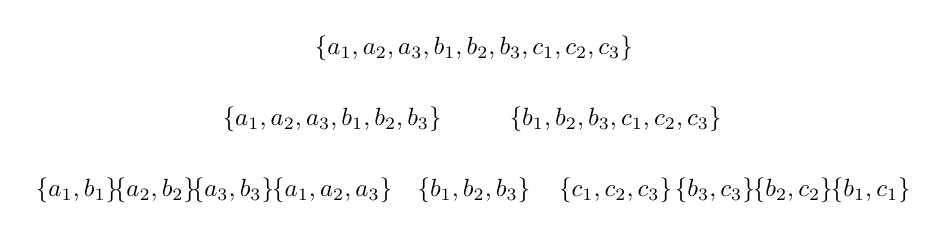
\begin{tikzpicture}[scale=.9, transform shape]
    \tikzstyle{v}=[draw, circle, minimum size=0.75cm, font=\footnotesize]
    % \tikzstyle{b}=[draw, font=\footnotesize]
    \tikzstyle{b}=[]
    \tikzstyle{e}=[]

    \node[b] (c0) at (0,0) {$\{a_1,a_2,a_3,b_1,b_2,b_3,c_1,c_2,c_3\}$};
    \node[b] (c1a) at (-2,-1) {$\{a_1,a_2,a_3,b_1,b_2,b_3\}$};
    \node[b] (c1b) at (2,-1) {$\{b_1,b_2,b_3,c_1,c_2,c_3\}$};
    \node[b] (c2a) at (-2,-2) {$\{a_1,a_2,a_3\}$};
    \node[b] (c2b) at (0,-2) {$\{b_1,b_2,b_3\}$};
    \node[b] (c2c) at (2,-2) {$\{c_1,c_2,c_3\}$};
    \node[b] (c2ab1) at (-5.6,-2) {$\{a_1,b_1\}$};
    \node[b] (c2ab2) at (-4.5,-2) {$\{a_2,b_2\}$};
    \node[b] (c2ab3) at (-3.4,-2) {$\{a_3,b_3\}$};
    \node[b] (c2bc1) at (5.6,-2) {$\{b_1,c_1\}$};
    \node[b] (c2bc2) at (4.5,-2) {$\{b_2,c_2\}$};
    \node[b] (c2bc3) at (3.4,-2) {$\{b_3,c_3\}$};

    \tedge{c0}{c1a}{solid}{}{};
    \tedge{c0}{c1b}{solid}{}{};

    \tedge{c1a}{c2ab1}{solid}{}{};
    \tedge{c1a}{c2ab2}{solid}{}{};
    \tedge{c1a}{c2ab3}{solid}{}{};
    \tedge{c1a}{c2a}{solid}{}{};
    \tedge{c1a}{c2b}{solid}{}{};

    \tedge{c1b}{c2bc1}{solid}{}{};
    \tedge{c1b}{c2bc2}{solid}{}{};
    \tedge{c1b}{c2bc3}{solid}{}{};
    \tedge{c1b}{c2b}{solid}{}{};
    \tedge{c1b}{c2c}{solid}{}{};
\end{tikzpicture}

%     \caption{}\label{fig:doublets:b}
% \end{subfigure}

% \caption{(\ref{fig:doublets:a}) Two doublets ($C_2\times C_3$), $\{a_1,a_2,a_3,b_1,b_2,b_3\}$ and $\{b_1,b_2,b_3,c_1,c_2,c_3\}$, intersecting on the triangle $\{b_1,b_2,b_3\}$. (\ref{fig:doublets:b}) The optimal DR-plan of the graph if we consider it to be a 2D graph; omits further decomposition of the three triangles into their edges and of edges into their individual nodes.}
% \label{fig:doublets}
% \end{figure*}


% \myexample
% In figure \ref{fig:doublets}, the two well-constrained vertex-maximal proper subgraphs of the graph are the two doublets, shown in the second level of the DR-plan. These intersect on the well-constrained graph $\{b_1,b_2,b_3\}$. This will necessarily be a child $N=2$ levels below the parent of the two doublets, as explained in Theorem \ref{theorem:main}, point 1. Also shown is the decomposition of the individual doublets. These have five well-constrained vertex-maximal proper subgraphs, the two triangles and the three edges connecting them. As explained in Theorem \ref{theorem:main}, point 2, all of them must be included in the optimal DR-plan. Were any left out, the union of the children would not be the entire parent.



\begin{figure*}\centering
\begin{subfigure}{.3\linewidth}\centering
    % \newcommand{\tedge}[5]{\draw[#3] (#1)-- node[e, #5] (e#4) {#4} (#2)}

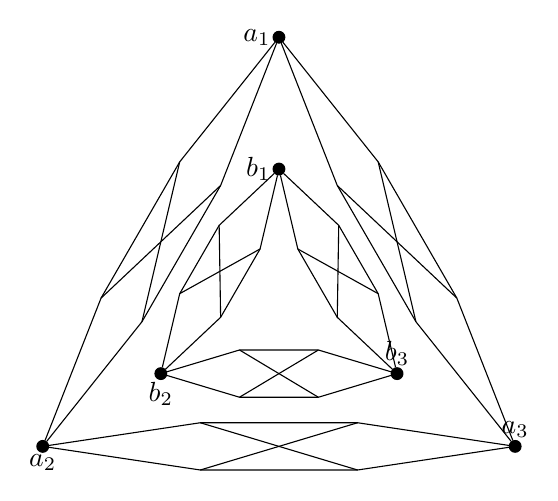
\begin{tikzpicture}[scale=3]
    \tikzstyle{v}=[draw, circle, minimum size=0.75cm]
    \tikzstyle{c}=[draw, circle, inner sep=1.5, fill=black]
    \tikzstyle{e}=[]

    \node[circle,fill=white,inner sep=7] (center) at (0,0-.125-.1) {};

    \node[c] (v1) at (0,0.866) [label={left,inner sep=.555}:$a_1$]{};
    \node[c] (v2) at (-1,-0.866) [label={below,inner sep=.555}:$a_2$]{};
    \node[c] (v3) at (1,-0.866) [label={above,inner sep=.555}:$a_3$]{};

    \node[c] (v4) at (0,0.433-.125) [label={left,inner sep=.555}:$b_1$]{};
    \node[c] (v5) at (-0.5,-0.433-.125) [label={below,inner sep=.555}:$b_2$]{};
    \node[c] (v6) at (0.5,-0.433-.125) [label={above,inner sep=.555}:$b_3$]{};

    \tedge{v1}{v2}{solid}{}{};
    \tedge{v1}{v3}{solid}{}{};
    \tedge{v2}{v3}{solid}{}{};

    \tedge{v4}{v5}{solid}{}{};
    \tedge{v4}{v6}{solid}{}{};
    \tedge{v5}{v6}{solid}{}{};


    \tedge{v1}{v4}{solid}{}{};
    \tedge{v2}{v5}{solid}{}{};
    \tedge{v3}{v6}{solid}{}{};


    \tedge{v4}{center}{dashed}{}{};
    \tedge{v5}{center}{dashed}{}{};
    \tedge{v6}{center}{dashed}{}{};


    % sin(30deg) = 0.5
    % cos(30deg) = 0.866

    % o/i -> outside/inside triangle
    % b/l/r -> bottom/left/right edge of triangle

    \coordinate (ob0) at (-0.333,-0.866-0.1);
    \coordinate (ob1) at (0.333,-0.866-0.1);
    \coordinate (ob2) at (-0.333,-0.866+0.1);
    \coordinate (ob3) at (0.333,-0.866+0.1);
    \draw (v2) -- (ob0) -- (ob1) -- (v3);
    \draw (v2) -- (ob2) -- (ob3) -- (v3);
    \draw (ob0) -- (ob3);
    \draw (ob2) -- (ob1);

    \draw[rotate around={60:(-1,-0.866)}] (v2) -- (-0.333,-0.766) -- (0.333,-0.766) -- (v1);
    \draw[rotate around={60:(-1,-0.866)}]  (v2) -- (-0.333,-0.966) -- (0.333,-0.966) -- (v1);
    \draw[rotate around={60:(-1,-0.866)}]  (-0.333,-0.766) -- (0.333,-0.966);
    \draw[rotate around={60:(-1,-0.866)}]  (-0.333,-0.966) -- (0.333,-0.766);

    \draw[rotate around={-60:(1,-0.866)}] (v3) -- (0.333,-0.766) -- (-0.333,-0.766) -- (v1);
    \draw[rotate around={-60:(1,-0.866)}]  (v3) -- (0.333,-0.966) -- (-0.333,-0.966) -- (v1);
    \draw[rotate around={-60:(1,-0.866)}]  (-0.333,-0.766) -- (0.333,-0.966);
    \draw[rotate around={-60:(1,-0.866)}]  (-0.333,-0.966) -- (0.333,-0.766);




    \coordinate (ib0) at (-0.167,-0.433-.125-0.1); %(-.167,-.658)
    \coordinate (ib1) at (0.167,-0.433-.125-0.1); %(.167,-.658)
    \coordinate (ib2) at (-0.167,-0.433-.125+0.1);%(-.167,-.458)
    \coordinate (ib3) at (0.167,-0.433-.125+0.1);%(.167,-.458)
    \draw (v5) -- (ib0) -- (ib1) -- (v6);
    \draw (v5) -- (ib2) -- (ib3) -- (v6);
    \draw (ib0) -- (ib3);
    \draw (ib2) -- (ib1);

    \draw[rotate around={60:(-0.5,-0.558)}] (v5) -- (-.167,-.658) -- (.167,-.658) -- (v4);
    \draw[rotate around={60:(-0.5,-0.558)}]  (v5) -- (-.167,-.458) -- (.167,-.458) -- (v4);
    \draw[rotate around={60:(-0.5,-0.558)}]  (-.167,-.658) -- (.167,-.458);
    \draw[rotate around={60:(-0.5,-0.558)}]  (-.167,-.458) -- (.167,-.658);

    \draw[rotate around={-60:(0.5,-0.558)}] (v6) -- (.167,-.658) -- (-.167,-.658) -- (v4);
    \draw[rotate around={-60:(0.5,-0.558)}]  (v6) -- (.167,-.458) -- (-.167,-.458) -- (v4);
    \draw[rotate around={-60:(0.5,-0.558)}]  (-.167,-.658) -- (.167,-.458);
    \draw[rotate around={-60:(0.5,-0.558)}]  (-.167,-.458) -- (.167,-.658);
% \newcommand{\tedge}[5]{\draw[#3] (#1)-- node[e, #5] (e#4) {#4} (#2)}

    % \draw (-1,-0.866) -- (-0.333,-0.966);

\end{tikzpicture}

    \caption{}\label{fig:c2c3ofk33s:a}
\end{subfigure}%
\begin{subfigure}{.7\linewidth}\centering
    % \newcommand{\tedge}[5]{\draw[#3] (#1)-- node[e, #5] (e#4) {#4} (#2)}

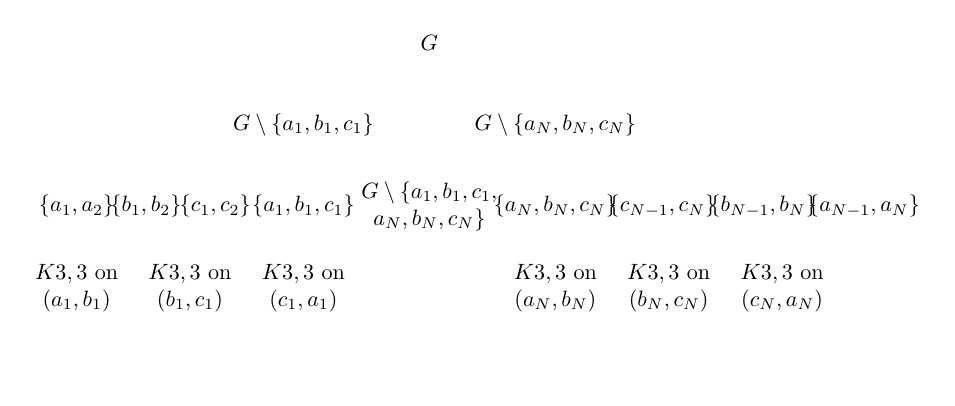
\begin{tikzpicture}[scale=.8, transform shape]
    \tikzstyle{v}=[draw, circle, minimum size=0.75cm, font=\footnotesize]
    % \tikzstyle{b}=[draw, font=\footnotesize]
    \tikzstyle{b}=[align=center]
    \tikzstyle{e}=[]

    \node[b] (c0) at (0,0*1.3) {$G$};
    \node[b] (c1a) at (-2,-1*1.3) {$G\setminus\{a_1,b_1,c_1\}$};
    \node[b] (c1b) at (2,-1*1.3) {$G\setminus\{a_N,b_N,c_N\}$};
    \node[b] (c2b) at (0,-2*1.3) {$G\setminus\{a_1,b_1,c_1,$ \\ $a_N,b_N,c_N\}$};
    \node[b] (c2a) at (-2,-2*1.3) {$\{a_1,b_1,c_1\}$};
    \node[b] (c2c) at (2,-2*1.3) {$\{a_N,b_N,c_N\}$};
    \node[b] (c2ab1) at (-5.6,-2*1.3) {$\{a_1,a_2\}$};
    \node[b] (c2ab2) at (-4.5,-2*1.3) {$\{b_1,b_2\}$};
    \node[b] (c2ab3) at (-3.4,-2*1.3) {$\{c_1,c_2\}$};
    \node[b] (c2bc1) at (6.9,-2*1.3) {$\{a_{N-1},a_N\}$};
    \node[b] (c2bc2) at (5.3,-2*1.3) {$\{b_{N-1},b_N\}$};
    \node[b] (c2bc3) at (3.7,-2*1.3) {$\{c_{N-1},c_N\}$};

    \node[b] (ab1k33) at (-5.6,-3*1.3) {$K3,3$ on \\ $(a_1,b_1)$};
    \node[b] (bc1k33) at (-7.6/2,-3*1.3) {$K3,3$ on \\ $(b_1,c_1)$};
    \node[b] (ca1k33) at (-2,-3*1.3) {$K3,3$ on \\ $(c_1,a_1)$};

    \node[b] (abNk33) at (2,-3*1.3) {$K3,3$ on \\ $(a_N,b_N)$};
    \node[b] (bcNk33) at (7.6/2,-3*1.3) {$K3,3$ on \\ $(b_N,c_N)$};
    \node[b] (caNk33) at (5.6,-3*1.3) {$K3,3$ on \\ $(c_N,a_N)$};


    \node[b] (c3a) at (-2,-4*1.3) {};
    \node[b] (c3b) at (2,-4*1.3) {};


    \tedge{c0}{c1a}{solid}{}{};
    \tedge{c0}{c1b}{solid}{}{};

    \tedge{c1a}{c2ab1}{solid}{}{};
    \tedge{c1a}{c2ab2}{solid}{}{};
    \tedge{c1a}{c2ab3}{solid}{}{};
    \tedge{c1a}{c2a}{solid}{}{};
    \tedge{c1a}{c2b}{solid}{}{};

    \tedge{c1b}{c2bc1}{solid}{}{};
    \tedge{c1b}{c2bc2}{solid}{}{};
    \tedge{c1b}{c2bc3}{solid}{}{};
    \tedge{c1b}{c2b}{solid}{}{};
    \tedge{c1b}{c2c}{solid}{}{};

    \tedge{c2a}{ab1k33}{solid}{}{};
    \tedge{c2a}{bc1k33}{solid}{}{};
    \tedge{c2a}{ca1k33}{solid}{}{};
    \tedge{c2c}{abNk33}{solid}{}{};
    \tedge{c2c}{bcNk33}{solid}{}{};
    \tedge{c2c}{caNk33}{solid}{}{};

    \tedge{c2b}{c3a}{dashed}{}{};
    \tedge{c2b}{c3b}{dashed}{}{};
\end{tikzpicture}

    \caption{}\label{fig:c2c3ofk33s:b}
\end{subfigure}

\caption{(\ref{fig:c2c3ofk33s:a}) A doublet ($C_2 \times C_3$) with each edge of the triangles replaced by a $K_{3,3}$. This pattern continues inwards for a total of $N$ triangles, indicated by the dashed lines. (\ref{fig:c2c3ofk33s:b}) Most of the DR-plan of this graph, omitting further decomposition of $K_{3,3}$ subgraphs into the separate 9 edges and of edges into the component nodes. $G\setminus\{a_i,b_i,c_i\}$ is shorthand for $G$ difference those nodes and all of the nodes in the corresponding $K_{3,3}$ subgraphs. The dashed lines indicated that this exact structure is repeated.}
\label{fig:c2c3ofk33s}
\end{figure*}

\myexample
\textsl{[DR-Plan for self-similar structure]}
This section details the decomposition of the graph in Figure \ref{fig:c2c3ofk33s}. The graph $G$ has only two isostatic vertex-maximal subgraphs, $G$ without the outermost triangle composed of $K_{3,3}$ graphs (triangle $1$) and $G$ without the inner triangle $N$. These intersect on $G$ without triangle $1$ and $N$ which is clearly well-constrained. As explained in the proof of Theorem \ref{theorem:main}, part 2, since there are only 2 possible children, their intersection must be a node 2 levels below the parent. Just as expected, it is on the third level, as it is a child of both of $G$'s children. Furthermore, it intersects trivially with the edges that connect triangle $1$ and $N$ to $2$ and $N-1$, respectively; these necessarily intersect with triangle $1$ and $N$ themselves trivially (by Theorem \ref{theorem:main}, part 1) making all of these children. The triangles then decompose into their constituent $K_{3,3}$ graphs, which then decompose into 9 edges.

Now, the self-similar nature of the graph is clear; $G$ without triangle $1$ and $N$ has the same structure, and thus the same pattern is repeated until only triangle $(N+1)/2$ remains in the case that $N$ is odd, or until only triangles $N/2$ and $N/2+1$ remain if $N$ is even.


% \begin{example}
%     In
% \end{example}




% \subsection{Extensions}
% This framework immediately pushes through for body-pin systems via a simple reduction. If there are $N$ pins on a body, it can be represented as a 2-tree with $N$ vertices, each corresponding to a pin, making sure to select edge distances such that the distance between pins is preserved. E.g.\ a body with two pins is an edge, three pins is a triangle, etc. Any bodies that share a pin now intersect on their vertex that corresponds to that pin. Now we have a bar-joint representation of the body-pin system in 2D and all proofs follow.

% With more effort, it can be shown that pinned line-incidence systems can also use this framework. This is done in section \ref{XXX}.


\subsection{Algorithm}

The first step of the algorithm to find an optimal DR-plan is the most difficult --- to find the well-constrained vertex-maximal proper subgraphs of the input well-constrained graph. There are two approaches: (1) the bottom-up approach, using the Frontier algorithm \cite{Oung:2001:FFE:376957.376995} to grow these components from single vertices; and (2) the top-down approach, using the pebble game algorithm \cite{Jacobs:1997:PG} on each node and taking the largest components that are not subgraphs of any larger ones. After the subgraphs have been found, it is a straightforward application of the theory. If the intersection of any two of the subgraphs is well-constrained, then take those two to be children of the graph. Otherwise, all the subgraphs are the children. Apply recursively to the children. This naturally terminates when you reach trivial subgraphs. The complexity of this depends on the algorithm for finding children (both are polynomial) and the depth of the plan (the deeper the plan, i.e.\ the smaller the max fan-in, the longer the running time). \todo{Think more about complexity.}
